\documentclass{beamer}
\usepackage{xcolor}
\usepackage[utf8]{inputenc}
\usepackage{pifont}
\usepackage{multimedia}
\usepackage{listings}             % Include the listings-package
\usepackage{subcaption}
\usepackage{tikz}
\mode<presentation>						% Set options
{
  \usetheme{Madrid}					% Set theme
  %\usecolortheme{default} 				% Set colors
  %\usefonttheme{default}  				% Set font theme
  \setbeamertemplate{caption}[numbered]	% Set caption to be numbered
  \setbeamertemplate{footline}[frame number]
}

\AtBeginSection{
\begin{frame}[plain]{Plan de la soutenance}
\tableofcontents[currentsection]
\end{frame}
}

\title{Développement évolutionnaire de systèmes de systèmes avec une approche par patron de reconfiguration dynamique}
\author{PETITDEMANGE Franck}
\institute{
\includegraphics[scale=0.15]{logo_irisa.jpg}}
\date{le 3 décembre 2018}

\begin{document}

\captionsetup[figure]{labelformat=empty}

\begin{frame}[plain]
\titlepage
\begin{center}
Directrice : BORNE Isabelle\\
Co-directeur : BUISSON Jérémy  
\end{center}

\end{frame}

\section{Introduction}

\subsection{Titre}
Je vais présenter ma thèse intitulé "Développement évolutionnaire de
SdS avec une approche par patron de reconfiguration" 

\subsection{Diapo 2}
\paragraph{}
Des exemples de SdS sont par exemple :
Des systèmes de surveillance d'inondation ou les capteurs collaborent
momentannement pour calculer des informations environnementales

Les services de secours. Les composants sont les services de secours.
Chacune d'elle possède sa propre indépendance managériale puisqu elle
dispose de ces propres ressources et définit elle même sont
organisation interne. Chaque système possède sa propre indépendance
oéprationnelle car ils peuvent réaliser leur mission indépendamment
des autres. Les pompiers peuvent faire de lutte contre les incendies
et faire du secours à personne sans l'aide des autres. Par contre
l'intéraction avec les autres systèmes peut améliorer la mission de 
chaque service de secours. Par exemple, la police peut sécuriser et
faciliter l'accès des pompiers à un sinistre.

Internet où les composants sont des routeurs qui implémentent le
protocole ip et collabore volontairement 

Le Web ou les composants sont les services web dont la composition
fournissent d'autres services. 
\paragraph{}
Les SdSs sont une
classe système dont les constituants sont eux mêmes des
systèmes. Les SdSs héritent des caractéristiques des systèmes
distribués car
leur composant sont géographiquement distribué. Mais ce qui les
différencie de système distribué est que leurs consistuants possèdent
leur propre
indépendance managérialle et opérationnelle. La raison de la
collaboration entre ces systèmes est le comportement emergent produit.
C'est un comportement qui ne peut pas être réalisé par un seul des
constituants du SdSs et qui apporte en général un bénéfice à tous les
participants au SdS.


\paragraph{}
Parmis les SdSs, on peut distinguer plusieurs catégories de SdS
suivant le niveau coercitif sur ses composants à prendre en compte 
dans leur ingénirie.
Les réseaux de capteurs malgrès qu'ils peuvent opérer indendamment du
SdS ont des objectifs de collaboration imposés.

Les services de secours sont plutôt un SdS consensuel car les
objectifs du SdS sont décidés de façon consensuel.

Internet définit des objectifs de routage mais l'implication des
composants reste volontaire.

Le web les objectifs ne sont pas idenifier et la collaboration est la
collaboration est volontaire.

\paragraph{}
Dans la thèse, on a étudieé plutôt les systèmes consensuels. Sans
donner un importance particulière à la catégorie de SdS. Ce qui nous a
particulierement interessé est la conséquence de l'ensemble de ces
catéristiques qui est le développement évolutionnaire du sds. 


\subsection{Diapo 3}
\paragraph{}
On a considéré que le développement évolutionnaire est l'évolution
permanente des buts et fonctions du SdS pendant sont execution. 

\paragraph{} 
La cause du développement évolutionnaire est qu'au moment de la
conception, le SdS ne connaît pas toutes les informations sur
l'environnement d'execution au moment de la conception. 

Les raisons peuvent être est managériale, les consituants évoluent en
changeant eux mêmes est les services fournit dans SdS sont impactés.
Le SdS doit s'accomoder des capacités de ses constituants qui peuvent
changer. 

Des SdSs sont formés momentanement en réaction à un événement dont
toutes les informations ne sont pas connu au moment de la conception
et découvertes seulement pendant la phase d'execution.    


\paragraph{}
Pour toutes ces raisons, le SdS est améné à évoluer régulierement
après la phase de conception et de déploiement. Ce qui nécessite des
outils particuliers pour assister l'architecte du SdS afin de maîtriser au
mieux le développement évolutionnaire. 
  
\subsection{Diapo 4}

\paragraph{}
Comme solution les SdSs sont amanés à intégrer régulierement de plus
en plus de logiciel pour supporter le developpement évolutionnaire et
en particulier au niveau de la phase de conception de l'architecture
des SdSs.

Dans notre thèse on a pris comme référénce deux
projets européens qui sont DANSE et COMPASS. On peut remarquer la
pré-pondérance du logiciel dans le processus de conception de
l'architecture des SdS.
Les phases de conception intègre des générateur d'architecture, 
des outils de simulation pour la vérification et divers langage pour
modéliser les objectifs du SdS, les contraintes à respecter dans les
architecture et la description du comportement des systèmes
consitituants. 

\paragraph{} 
Un aspect du cycle de vie des systèmes moins étudié pour les SdSs est
la phase de déploiement de la nouvelle architecture dynamiquement et que nous avons
abordé en particulier dans cette thèse à travers le problème de la
reconfiguration dynamique.

\subsection{Diapo 5}

\paragraph{}
La reconfiguration dynamique consiste donc à apporter des
modifications sur un système pendant qu'il s'execute. Ces
modifications peuvent être corrective, fonctionnelle si il s'agit
d'ajouter une fonctionnalité, non fonctionnelle si elle modifie la
qualité du système.  La difficulté réside dans la maîtrise des parties
du système interrompue, les dégradations de services, l'intégrité du
système pendant le temps de la reconfiguration. 

\paragraph{}
De manière générale, la reconfiguration dynamique vient du besoin de
pouvoir appliquer des modifications à un système sans le redémarrer
complétement. Dans un contexte SdS, c'est particulierement intéressant
car les SdSs sont typiquement des systèmes qui une fois déployés ne
peuvent pas être arretés puis redemarrés. Les risques seraient suivant
le sds : économique et/ou humaine. 
 
\paragraph{} 
Comme solution à la reconfiguration dynamique nous proposons
d'outiller l'architecte pour l'assister face au développement
évolutionnaire des SdSs. 

\subsection{Diapo 6}

\paragraph{} 
Pour adresser un problème de reconfiguration l'architecte doit être
capable de communiquer ses choix de conception dans un but de
validation par ces pairs pour améliorer et valider une
reconfiguration. Ensuite les solutions doivent être capitalisées pour
résoudre plus facilement des problèmes similaires déjà résolus. C'est
un gain de temps et de fiabilité des solutions de conception proposée. 
mêmes erreurs. 

\paragraph{}
Comme solution on propose d'intégrer la notion de patron de conception
bien connu dans la domaine logiciel. Les patrons de conception sont
une solution documentée face à un problème récurrent. Les patrons de
conceptions les plus connus sont ceux du GoF, ils sont utilisés dans
la programmation orientée objet pour favoriser la réutilisation du
code. L'exemple est repris dans d'autres champs du logiciel comme la
conception d'architecture pour intégrer des aspects non fonctionnelles
comme la scalabilité ou l'adaptabilité. 

\paragraph{}
Une première difficulté a été l'étude de SdS pour identifier des
problème de reconfiguration que l'on pourrait rencontrer lors de
reconfiguration. Dans l'état de l'art des SdSs peu d'étude de cas se sont intéressées
à capturer des configurations résultantes d'évolutions successives et
des propriétés de reconfiguration souhaitées.

\subsection{Diapo 7}

\paragraph{}
Le challenge à été de capturer des configurations avec le niveau de
précision suffisant pour capturer des propriétés de reconfiguration à
étudier mais aussi avec un niveau d'exactitude correcte pour capturer
des contextes de reconfiguration. 
%\paragraph{} 

\paragraph{}
Une dernière difficulté à été de determiner le processus de
reconfiguration à utiliser pour mettre en \oe{}uvre le concept de patron de
reconfiguration.

\subsection{Diapo 8} 
\paragraph{} 
Dans l'état de l'art on a constaté que la reconfiguration dynamique a
été principalement étudié du point de vue des langages pour la
décrire, des propriétés des protocoles de reconfiguration et
l'automatisation des protocoles de reconfiguration. 

%\section{Framework pour la modélisation des SdSs}

\subsection{Diapo 12}
\paragraph{à déplacer}
On a vu qu'une problématique de cette thèse a été la modélisation
d'architecture de SdSs nécessaire à l'étude de la reconfiguration
dynamique.
%
Le besoin ... 
%
Les modèles d'une manière générale sont des abstractions de la
réalité. 
%
En génie logiciel, il capture l'architecture du SdS. 
Ils sont utilisés pour améliorer la qualité et le cout des systèmes. On
peut réduire les cout et augmenter qualité par exemple avec
l'utilsiation des modèles pour générer automatiquement l'architecture
d'un système, faire des simulations pour améliorer la qualité de
l'architecture avant de la déploiyer. 

\paragraph{}
Un objectif de modélisation des SdSs est d'obtenir des modèles
exactes et précis. 
%exactitude
Ce qui nous interesse est de réussir à modéliser les abstractions qui
concour à la réalisation du SdS. On s'est interessé en particulier à
identifier tous les CSs et les ressources qu'ils déploient ainsi que
leurs objectifs d'interaction.
%précision
On aura besoin de modèle suffisament précis pour modéliser les
décisions
architecturales du SdS.

\paragraph{}
La problématique est un contexte de modélisation difficile dû  aux frontières du SdS flou.
Les frontères sont flou car les composants du SdS sont développés par
des tiers. Si on regarde la figure, si le SdS définit ses frontières
aux composants A,B, et C, il ne prend pas en compte D qui si il se
désengage de A et C peut dégrader fortement le fonctionnement global
du SdS.  

\paragraph{}
Parmis les études de cas disponibles peu s'intèressent à la
reconfiguration dynamique mais plutôt à la conception des
architectures. On s'est plutôt intéressé au langage et processus de
modélisation mis en \oe{}vre dans les études de cas. 
%
Pour la conception des systèmes complexes comme les sdss les langages
de modélisation ont été développé pour gérer la compléxité des
modèles, la précision et l'exactitude. Dans cette section, nous allons
étudier les langages de modélisation dans le developpement des SdSs et
leur portée. On définira leurs caractéristiques utiles et comment
elles sont exploiter dans les conceptions des SdS à travers deux
projets Europééens qui sont DANSE et COMPASS.


\subsection{Diapo 13}
\paragraph{}
Un premier langage de modélisation auquel on s'est intéressé est
SySML. C'est un langage de modélisation qui a l'ambition de permettre
une approche de modélisation holistique. L'idée est que le langage
puisse supporter toute les phases de développpement du SdS, notamment
en intégrant tous les corps de métier qui peuvent intervenir dans le
développement d'un système. 

\paragraph{}
Les principaux éléments de modélisation utilisés sont la notion de
block et de port. 
Les blocks modélisent des unités modulaires d'un système. 
Les ports décrivent les points d'intercation entre les blocs. Il y
plusieurs catégorie de port qui peuvent permettre de modéliser des
interactions entre des parties logicielles et matérielles. 
Ensuite les flux ajouter une description physique des interactions
entre les blocs. 
Pour finir la relation d'allocation permet de modéliser des relations
de raffinement entre les éléments modéliser ce qui est utile pour
supporter les processus de modélisation descendant ou ascendant. 

\paragraph{à déplacer} Plusieurs type de diagramme interviennent : les
diagrammes de block, d'interaction, d'activité, paramétrique,
d'exgience. 

\paragraph{} Les avantages pour la modélisation des systèmes de
systèmes sont la description des connectivités puisque la modélisation
des SdSs s'interessent à la description des interactions entre les
CSs, et traçabilité entre les éléments de modélisation qui permet
de définr des relations entre des modèles developpé à différent niveau
d'abstraction et/ou différent aspect, ce qui est un avantage des SdSs
qui intègre différent parti prennant dans la modélisation des SdSs. 

\paragraph{} Evidemment l'inconvénient est l'absence de parti pris
sur le type des éléments à modéliser. Des frameworks de modélisation
Comme UPDM peuvent vu comme des profils de SySML est proposer des
modèles pour le developpement des SdSs. 

\subsection{Diapo 14} 
\paragraph{}
un second langage que l'on a étudié est UPDM. UPDM est profil de
SysML. Sa principale contribution est la proposition de 40 vue pour la
modiélisation de SdS. 

\paragraph{}
Différent type de vue propose de modéliser des niveaux d'abstraction
différent :
\begin{itemize}
\item Les vues Acquisition / Project (AcV / PV) décrivent les aspects
organisationnels
des projets, y compris leur calendrier et les jalons.
\item Les All-Views (AV) rassemblent des informations globales et des
métadonnées sur
les éléments de l’architecture.
\item Les vues opérationnelles (OV) sont une collection de vues qui
décrivent les activités
impliquées dans le SdS, ainsi que les ressources (humaines ou
mécaniques) qui
exécutent ces activités.
\item Les vues orientées services (SOV) décrivent les services, en termes
d’interfaces,
ainsi que les fonctions que les services sont censés exécuter dans le
but de mettre
en œuvre les activités décrites dans les vues opérationnelles.
\item Les vues stratégiques / de capacités (StV / CV) sont un ensemble de
vues à
long terme croisées entre projets qui décrivent et organisent les
capacités d’une
organisation, en prévision de projets.
\item Les vues système / services (SV / SvcV) sont une collection de vues
qui décrivent
comment les capacités opérationnelles, décrites dans les vues
opérationnelles, et
les exigences des utilisateurs peuvent être réalisées en termes de
capacités d’équi-
pement (ou humain), c’est-à-dire la spécification des constituants
impliqués dans
le système.
\item Les vues techniques / standards (TV / StdV) décrivent les
technologies, les règles
et les normes qui sous-tendent la mise en œuvre du système,
fournissant ainsi un
outil pour anticiper les progrès technologiques ou les perturbations
qui peuvent
affecter le système. 
\end{itemize}

\paragraph{}
Concretement on a regardé leur utilisation pour définir leur portée et
comment ils sont utilisés.  Pour cela on a étudié les principaux
projets de recherche européen
dans le domaine de SdSs. Il s'agit de DANSE. qui a basé sont projet
developpemment de SdS sur le langage UPDM. 

\paragraph{} 
Le tableau fait la synthèse des vues et diagrammes selectionnées par
danse.
 
Si on regarde leur utilisation, les vues opérationnelles servent à
identifier .... 

les vues systèmes servent à ...

\paragraph{}
après la phase de modélisation avec UPDM, les modèles sont raffinés
vers des représentation plus formelles. définition des contrats sur
l'architecture comme objectif à optimiser pour générer une architecture, 
la vue sv-1 assiste la génération d'architecture automatique.
définition de contrainte de cout à respecter, ...

les vues sv-4 servent à analyse les evolutions de possible du SdS.
définition de relation de causalité et probabilité de réalisation. 
+ Définition de contrat sur les CSs 

\paragraph{}
Si on regarde en comparaison le framework developpé par compass, les
vues developpées sont similaire.
 
\paragraph{}
A ce stade on voit que l'exactitude est obtenu grâce à un processus de
développement descendant. La modélisation démarre par des abstractions
hauts niveaux qui capture les systèmes participants et les objectifs
d'interaction. Puis raffine sont raffiné vers des abstractions
concrètrs. 
Au niveau de la précision on a noté que SySML et UPDM ne sont pas
suffisant pour exprimer des propriétés vérifibles de façon automatique. 


\subsection{}

\paragraph{}
Dans notre approche de modélisation des architectures de SdSs on a
choisi de se baser sur l'existant. Sans proposer de modification des
profondes. En effet, en comparaison avec d'autres travaux de
modélisation que soit pas basé sur UPDM on voit que les vues et pts de
vue sont similaires. On a pris en parti pri que cela suffit pour le
moment à fournir des données réalistes. 


\paragraph{} 
On propose donc de suivre une approche top down pour la modélisation.
- On a ajouté une phase de modélisation des exigences pour les
structurer. 
- La phase de modélisation du niveau SdS repose sur les vues ov1, ov1b,
ov5.
- On a explicité une phase de validation manuel. 
- Puis une phase de modélisation de l'architecture au niveau CS.
- Puis une phase de vérification de la cohérence de l'architecture
avec une simulation. 

\paragraph{}
Si on regarde la modélisation du SdS on a retenu les vues OV-1, OV-1b,
OV4 et OV-5. 
%
On a rejoint le parti de DANSE, cependant on a trouvé plus
pertinent l'utilisation du diagramme de cas d'utilisation pour
modéliser les objectifs d'interaction entre les resssources. Cela
améliorer la lisibilité du diagramme et permet de guider le
developpement de la description des fonctions du SdS. Le détaille de
la connectivité modélisé avec OV2 dans DANSE description de la 
connectivité est décrite dans la vue OV-4.

\paragraph{} 
La phase de modélisation du niveau CS ...
ajout de contrainte ocl pour préserver l'expressivité du langage on a
opté pour l'utilisation de primitive architectural spécifié en ocl ce
qui nous a permis de l'intégrer directement dans la vue sv-1, utilisation de la sémantique du pi-calcul.

\paragraph{} 
A ce stade on a clarifié les choix de modélisation et les raisons.
Maintenant je vais expliquer configurations que l'on a choisi de
modéliser. 
\subsection{Diapo 17}
 
\paragraph{} 
On a choisi comme cas d'étude le système de service de secours
d'urgence. Le domaine du système est un cas typique de SdS. 

\paragraph{}
La mission principale sur laquelle se concentre notre cas d'étude est la
protection des personnes, des biens et de
l’environnement. Il peut s'agir du
transport d'une personne à l'hôpital, de limiter la progression d'une
inondation, d'un incendie ou de circonscrire une pollution fluviale. De manière
générale, un des objectifs de la mission est d'empêcher l'évolution d'un sinistre et de revenir à
une situation normale.   

\paragraph{} 
Les principaux cs sont : 
\begin{itemize}
%\item L'organe de contrôle principal est le Centre Opérationnel Départemental d'Incendie et de Secours (CODIS) qui traite les appels des victimes, supervise et coordonne l'ensemble des activités opérationnelles d'un service départemental d'incendie. Dans notre exemple deux centres d'opérations sont impliqués CODIS56 et CODIS35
\item Les hôpitaux prennent médicalement en charge  les victimes.
\item Les pompiers, à l'échelle départementale, sont structurés par un Service
Dépar\-te\-mental d'Incendie et de Secours (SDIS) qui possède ses
propres ressources maté\-rielles et sa propre structure de commandement.
Ce service est  responsable du transport des blessés, de la lutte contre les
incendies et de la protection des biens.  
\item Le  Service d'Aide Médicale
Urgente (SAMU) est le centre de régulation médicale d'urgence qui régule les
ressources de soins d'urgence (ambulances par exemple).
\item Enfin, la sécurité civile est impliquée dans des situations de crises majeures et peut fournir des moyens aériens.
\end{itemize}



\paragraph{} 
Au niveau du territoire français, les services de secours sont organisés par
département. Chaque type de service est déployé sur chaque département français
avec son propre financement et sa propre structure hiérarchique de commandement. La collaboration entre
les services est favorisée par le réseau
Il s'agit du
 réseau numérique de communications intra-services
(quand les communications sont limitées aux membres d'un même service) et inter-services (quand
les communications permettent à des membres de services différents de communiquer). Les
collaborations que peuvent former le sos ont des échelles différentes.
Elles peuvent être~: 
\begin{itemize}
\item Locales quand il s'agit de
communications entre deux ressources proches géographi\-quement. 
\item Départementales quand les ressources qui communiquent sont distribuées à l'échelle du
département. 
\item Inter-départementales quand ce sont des ressources de services appartenant
à deux départements différents.
\item Nationales quand elles impliquent des membres du gouvernement. 
\end{itemize} 

\paragraph{} 
Une gestion efficace consiste à
prendre les bonnes décisions au bon moment. Cette efficacité dépend de la
qualité des informations et du moment où elles sont fournies. Pour ces raisons
les services de secours se structurent autours d'une chaîne de
commandement. Les composants de la chaîne de commandement (qui sont les
ressources des services de secours) sont partionnés suivant leur niveau de
responsabilité décisionnaire. Ces niveaux de décision sont d'ordre : 
\begin{itemize}
\item Stratégique. Cela consiste à définir les objectifs et anticiper les besoins opéra\-tionnels en
réservant des ressources, afin de les allouer au moment opportun.
\item Tactique. Cela consiste à assigner des
objectifs aux ressources allouées
pour réaliser les objectifs stratégiques. 
\item Opérationnel. Cela consiste à décider d'opérations primitives dans le but
de réaliser les objectifs tactiques. 
\end{itemize}

La discipline hiérarchique impose aux composants de n'interagir qu'avec le niveau n+1 ou n-1. Lorsqu'il
s'agit d'interaction avec les composants du niveau n+1, ces interactions sont des remontées
d'information. Par exemple, les composants du niveau opérationnel font une
synthèse de la situation observée aux composants du niveau tactique. Les
communications vers le niveau n-1 concernent des directives. Par exemple, les
composants du niveau tactique décident de la zone de positionnement d'un
composant opérationnel et des actions qu'il doit réaliser. 
%
\paragraph{}
Cette chaîne de commandement se reflète dans la structure du réseau de
communication des pompiers. La communication entre le CODIS et ses
ressources déployées se fait principalement via
un canal de communication radio appelé canal opérationnel par le réseau ANTARES. Le canal opéra\-tionnel est un groupe de
communication déployé pour chaque SDIS. Chaque membre du groupe connecté
sur le même canal de communication peut écouter les messages envoyés par les autres
membres du groupe. On parle d'écoute passive. Via le canal opérationnel, le CODIS gère
toutes les interventions courantes en cours dans le département :
\begin{itemize}    
\item Les communications se font seulement de façon verticale. Par
exemple, un VTU ne peut pas communiquer avec un autre vtu.
\item Les abonnés ne prennent la parole que s'ils ont l'autorisation du CODIS et
s'il n'y a pas une autre communication en cours. Par exemple, le VTU demande
l'autorisation de parler avant d'envoyer son rapport. Un seul abonné peut avoir
la parole à un moment donné. 
\end{itemize}

D'autres types de canaux sont disponibles comme le canal tactique et
stratégique, pour les niveaux correspondants de la chaîne de commandement. Ces
canaux fonctionnent de la même manière que les canaux opérationnels, avec les mêmes contraintes.

\paragraph{}
La première configuration considère que deux sdis ont une collaboration
opérationnelle inter\-dé\-par\-tementale,
c'est-à-dire qu'ils communiquent directement, seulement pour ce qui concerne les
actions de terrain réalisées pour remplir la mission. Une telle collaboration
est mise en place, par exemple, lorsqu'un SDIS fait face à un manque de
personnel, et demande donc des ressources manquantes auprès d'un SDIS voisin
pour une mission de petite taille. Dans notre scénario, cette configuration est
utilisée lorsque les habitants appellent des services d'urgence en réponse à ce
que l'on pense être une inondation localisée.

\paragraph{}
Dans la deuxième configuration, deux SDIS ont une collaboration tactique et
stratégique interdepartementale, c'est-à-dire qu'une chaîne de commandement hiérarchique est mise en
place. En plus de la collaboration opérationnelle, la collaboration tactique
permet aux commandants de communiquer avec leurs subordonnés, afin de leur
donner des instructions et de recueillir des rapports sur les actions sur le
terrain. La collaboration stratégique garantit que le SDIS collaborateur adopte
des orientations cohérentes afin d'atteindre les objectifs de niveau supérieur
définis par la mission. Cette deuxième configuration est utilisée lorsque la
crise est plus importante, ce qui nécessite plus de ressources que dans la
première configuration, et lorsque ces ressources nécessitent une coordination
étroite. Dans notre scénario, le SdS évolue vers cette seconde configuration
lorsque les services d'urgence découvrent que l'inondation est plus critique
qu'ils ne le pensaient initialement.

\paragraph{}
Enfin, dans la troisième configuration, un SDIS collabore avec le SAMU et la
sécurité civile. Cette configuration se produit lorsque les services d'incendie
et de secours ont besoin de l'aide d'autres services pour faire face à la crise.
Dans notre scénario, le SAMU est impliqué afin de réguler l'évacuation des
blessés vers les hôpitaux les plus proches, et la sécurité civile fournit des
ressources de type hélicoptère lorsque l'inondation rend les routes
inutilisables.

\paragraph{} 
Maintenant que l'on a identifié des candidats à la modélisation, on
peut appliquer notre framework de modélisation. 


\subsection{Diapo }

\paragraph{}
étape 1 

\paragraph{}
étape 2 

\paragraph{}
étape 3 

\paragraph{}
étape 4 

\paragraph{}
étape 5 

\subsection{Diapo }

\paragraph{} 
A ce stade, nous avons modélisé 3 architectures qui correspondent à
la description d'environ ... composant/connecteur. et xx diagrammes.

Le processus de modélisation est supporté par le langage UPDM. On a vu
que UPDM n'est pas utilisable tel quel. il a fallu selectionné les
vues les plus pertinantes parmi la quarantaine disponibles. Pour
confirmer nos choix nous nous somme basé sur le choix de modélisation
d'autre étude de cas. 
%
Cela nous a permis d'expliciter des phases de
modélisation utilise. 
%
La modélisation des architectures reposent sur
l'utilisation de primitive architecturale ocl. L'avantage est
d'ajouter la précision nécessaire à une vérification automatique des
décisions architecturales. mais aussi d'assister la vérification de
l'exactitude de l'architecture en rendant plus expressif les
contraintes ocl. 

Cependant on peut noter tout de même que les modèles ne sont pas
complets  et pourrait être plus détaillés. 

\section{Patron et processus de reconfiguration}

\subsection{Diapo : Réutilisation de décision de reconfiguration}

Pour définir des critères de documentation réutilisables, on a fait la
synhtèse des parties descriptives des patrons de conception dans
l'état de l'art. On en en tirer la liste suivante. 
\begin{itemize}
\item titre
\item intention,
\item contexte, 
\item problème, 
\item solution 
\item conséquence.
\end{itemize} 

\paragraph{} 
Le titre et l'intention on pour objectif de donner l'intuiton du
principe mis en \oe{}uvre par la solution documentée. En général, le titre
correpond à une métaphore du principe suivi par la solution et
l'intention explique pourquoi une solution naive ne
fonctionne pas et quel est un principe plus adapté.   

\paragraph{} 
Le contexte va décrire quelles sont les hypothèses considérées par le
patron.  En somme, les pré-requis et les facteurs qui empêcheraient
l'application de la solution. 

\paragraph{} 
Le problème va expliquer quels sont les besoins que cherchent à
satisfaire la solution. et quelles sont les forces mise en \oe{}vre
par la solution. 

\paragraph{} 
Ensuite la solution documente comment est résolue le problème et enfin
les conséquences expliquent en générale quels sont les effets sur les
aspects non fonctionnels ou les considérations d'implémentation. 


\subsection{Diapo : Documentation formelle Allen}
On peut classifier le type de documentation suivant son niveau de
formalité. On a des documentations qui sont très formelles comme
celles utilisées par Allen ou Oliveira pour documenter des
reconfigurations. Ce niveau de formalisme permet de vérifier

%%%%
Si on regarde la proposition de Allen, il propose  de
réutilisation en considérant la phase de reconfiguration comme un
aspect à part dans le processus de developpement d'un système et donc
en proposant un langage et des outils dédiés à la reconfiguration
dynamique. 
%

\paragraph{} 
Il propose pas de patron en particulier. Si on regarde comment il
spécifie une reconfiguration. on voit que : 
%
\paragraph{} 
le contexte est définit par le langage WrightADL qui base sa
sémantique sur CSP. 
Le contexte se caractérise par une description composant/connecteur.
Ici on voit que contexte est décrit par une architecture
client/serveur.
%
\paragraph{} 
le problème est spécifié par des contraintes structurelles à respecter. pendant la
reconfiguration. On voit qu'un composant serveur doit toujours être connecté à
un composant client.  
%
\paragraph{} 
la solution est documenté par les événements qui déclenchent les
opérations de reconfiguration. On voit que lorsqu'un événement capture
que le serveur principal est hors service, la reconfiguration consiste
à déconnecter le client du serveur principal, vers le serveur
secondaire.
%
\paragraph{} 
les conséquences discuttent des aspects techniquent : notamment de
l'implémentation des événements et de la distribution du connecteur.  

formellement qu'une propriété est vérifiée pendant la reconfiguration. 

\subsection{Diapo : Documentation formelle}
%%%%%
\paragraph{} 
Si on regarde en détaille la proposition de Oliveira. 
%
Si on regarde les aspects réutilisations, elle concerne la description
d'opération de reconfiguration primitive récrruente et la description
formelle qui l'accompagne.  
%
\paragraph{} 
Le titre décrit directement l'opération appliquée.
%
\paragraph{} 
Par rapport à nos critère la reconfiguration est trop bas niveau pour
décrire une intention de reconfiguration. 
%
\paragraph{} 
le contexte est définit par la description de primitive de
reconfiguration. qui sont : constante, parallèlisation, union,
découpage, suppression 
%
\paragraph{} 
Le problème, il est décrit par l'architecture source et ciblée. mais
il y pas vraiment de contrainte à respecter.... si ce n'est qu'à la
fin l'architecture ciblée est atteinte.  
%
\paragraph{} 
la solution est documentée mais difficile à interpreter si
on ne connait pas le formalisme, de plus elle ne résoud pas de
problème particilier. 
%
\paragraph{} 
les conséquences ne sont pas
clairement documentées. comme le niveau est bas elle ne capture pas de
conséquence.   
%
\paragraph{} 
La réutilisation dans ce cas est partielle. Dans ce, c'est
prinpalement car les patrons sont trop bas niveau pour être
réutilisés. ils ne capturent pas de problème de conception. 

%%% 
\paragraph{} 
Les documentation consiste à considérer la reconfiguration
comme un aspect à part dans le developpement des systèmes. 
Donc considérer des langages et outil propre au
problème de reconfiguration. Ces langages assistent l'architecte pour
maintenir des propriétés pendant la reconfiguration. 

\subsection{Diapo : Documentation semi-formelle}
\paragraph{}
Si on regarde des approches moins formelles. Les travaux de Gomaa sont
plus intéressants. Les patrons de reconfiguration définissent une
solution de reconfiguration par rapport à un problème de
reconfiguration qui est la quiescence. 

\paragraph{}
Le titre du patron fait référence à contexte de reconfiguration et au
principe mis en \oe{}uvre. 

\paragraph{}
L'intention et le problème de la reconfiguration sont implicites ici
car les patrons ont tous pour objectifs de remplacer un composant avec
le principe de quiscence.

\paragraph{}
par rapport au documentation
précedente, on voit que le contexte est documenté par des digrammes de
collaboration qui montrent le rôle des composants dans l'architecture. 

Ensuite la solution est documentée via des diagrammes de collaboration qui
renseignent sur le rôle des composants entre eux. 

\paragraph{}
Par rapport à
l'approche précédente, la compréhension est simplifiée et elle ne
nécessite pas de connaissance pointue. 

\subsection{Diapo : }

\paragraph{}
A ce stade on voit que les approches comme celle de Gomaa sont du
point de vue de la réutilisation, une type de documentation plus
pertinent. 

\paragraph{}
On par rapport au critère de reconfiguration SdS, on voit que voit que
la solution de Gomaa est limité dans un contexte sds. en effet, on ne
peut pas faire l'hypothèse que les composants implémentent strictement
les mêmes mécanismes de reconfiguration. On veut proposer une
documentation qui prend en compte plus de type de décision de
reconfiguration. On voit que l'on aura besoin d'expliciter d'autres
champs pour notre concept de patron de reconfiguration.

\paragraph{}
Ensuite pour continuer notre approche de reconfiguration, on veut
s'intéresser au processus de reconfiguration que l'architecte a à sa
disposition dans l'état de l'art. 


 
\subsection{Diapo : Patron de reconfiguration - délimitation du problème}

\paragraph{}
Le problème de reconfiguration se réduit à la description du passage
d'une architecture à une autre. 
On peut cependant, raffiner en différent problème suivant les
solutions dévéloppés et en abstraire les régularités pour définir des
patrons de reconfiguration. 

\paragraph{}
On va essayer de déduire l'ensemble des besoins que cherche à
satisfaire la solution pour capturer le problème exprimer par le
patron. 
On a trouvé qu'un bon moyen est d'adord d'expimer l'architecture
intiale, puis celle ciblée. 
L'architecture est bon support pour la compréhension du problème lié à
qualité de service puisqu'elle modélise les dépendances fonctionnelles
enntre les composants. 

\paragraph{}
Ensuite on propose de documenter les contraintes que doivent satisfaire
la solution. Elles peuvent être structurelles ou comportementales.

\paragraph{}
Les forces doivent expliquer les principes mis \oe{}vre dans la
solution. Cela doit aider l'archticte à comprendre quelles sont les
points importants de la solution.  

%%ù
\paragraph{}
Dans la littérature, on a essayé d'analyser des solutions
récurrente. On a constaté qu'une solution consistait à appliquer des
reconfiguration graduellement. On a définit comme contexte
architectural ..., puis comme contrainte que ..., et force ...  

\subsection{Diapo : Patron de reconfiguration - rédaction de la solution}

\paragraph{}
Ensuite la solution consiste à décrire les mécanismes d'évolution
et d'une grammaire de reconfiguration. La grammaire de reconfiguration
consiste à  décrire les opérations de reconfiguration et leur ordre
afin de d'execution. Pour documenter la grammaire de reconfiguration
nous nous sommes appuyé sur des diagrammes de collaboration et d'état
ainsi qu'une description textuelle. 
 
\paragraph{}
On a documenté la reconfiguration à partir du schéma ... 
et d'une description textuelle ... qui indique la sémantique des
opérations. 

\subsection{Diapo : Patron de reconfiguration - amélioration de la
ré-utilisation}

\paragraph{}
Naturellement chaque solution à un impacte sur les aspects non
fonctionnels du système pendant la reconfiguration qui doivent être
documenté. 

\paragraph{}
Pour finir, la documentation doit permettre à l'architecte d'évaluer
rapidement la pertinence de la solution sans avoir à comprendre en
détail le patron de reconfiguration. Dans l'idée de titre des patrons, on a garder l'idée de la métaphore.

\paragraph{}
Dans la continuité du titre l'intention doit aboutir à la
comprenhension de la métaphore. en expliquant, un approche naive et
ses inconvénients puis on explique l'idée générale du patron et ses
avantages en comparaison avec l'approche naive. 
l'approche du patron  

\subsection{résumé } 

\paragraph{}
A ce stade on a identifié et documenté plusieurs patrons de
reconfiguration. On a donc la 

\begin{itemize}
\item quiescence : dont l'objectif le principe est de rendre passif,
les composants dépendant du composant ciblé par la reconfiguration. 
\item tranquilité : est une variante de la quiescence qui assouplie
les critères de reconfiguration. Elle décrit les conditions dans
lesquelles la reconfiguration pêtre réalisée sans attendre l'état de
tranquilité
\item co-evolution : contrairement à la quiescence et tranquilité, à
déployer directement la nouvelle version du composant ciblé par la
reconfiguration. La conséquence est que les deux versions d'un
composant s'execute simultanément. 
\item opportuniste : par rapport aux autres, il concerne une
granularité différente puisqu'il concerne seulement une opération de
déconnexion et connexion qui est réalisé dès que l'occasion se
présente.  
\end{itemize}





\section{Processus de reconfiguration} 

\begin{frame}{Processus de conception de reconfiguration existant}
\begin{figure}
\begin{subfigure}[b]{0.45\textwidth} % "0.45" donne ici la largeur
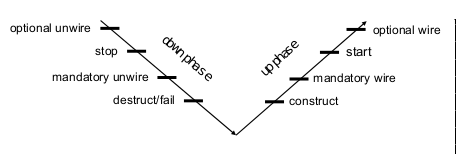
\includegraphics[width=5cm, height=3.8cm]{imgs/boyer_protocole}
\caption{Automatique, \emph{Boyer et al, 2017}}\label{fig:orchid}
\end{subfigure}
\begin{subfigure}[b]{0.45\textwidth} % "0.45" donne ici la largeur
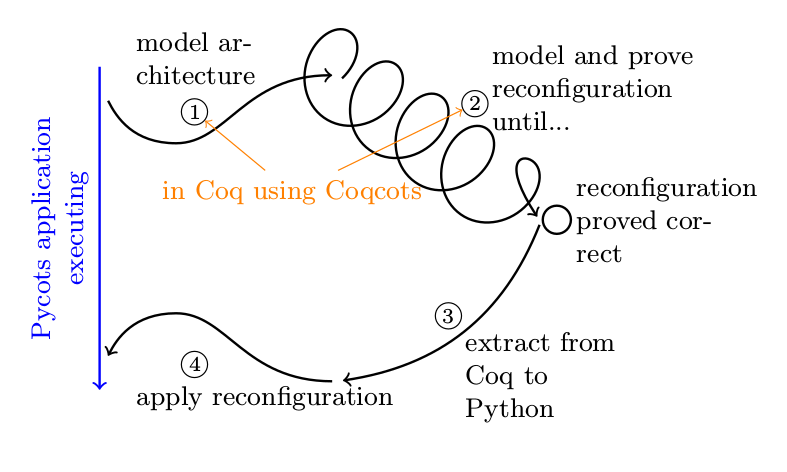
\includegraphics[width=5cm]{imgs/buisson_approche}\\
\caption{Manuelle \emph{Buisson et al, 2017}}\label{fig:orchid}
\end{subfigure}
\end{figure}
\end{frame}

\begin{frame}{Proposition d'un processus de reconfiguration}
\begin{figure}
\centering
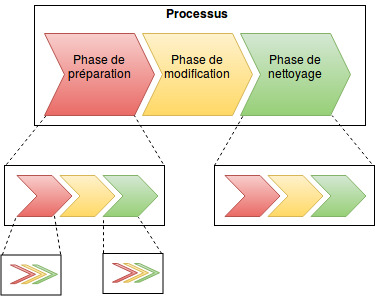
\includegraphics[width=8cm]{imgs/phases-de-reconfiguration.jpg}
\end{figure}
\end{frame}

\begin{frame}{Utilisation des patrons de reconfiguration}
Le processus s'appuie sur les patrons de reconfiguration. Dans un
premier temps, l'architecte analyse les modifications à apporter.\\

il utilise le catalogue de patron pour identifier les problèmes qu'il
peut rencontrer et comment les résoudre. ou il définit un nouveau
patron. \\

Dans le cas, ou le solution n'est pas directement applicable alors il
peut décider d'une nouvelle itération .
\end{frame}

\section{Expérimentation}
\begin{frame}{Framework de reconfiguration}
    
\end{frame}

\begin{frame}{Configuration de l'expérimentation}
    
\end{frame}

\begin{frame}{Formulation des hypothèses}
\end{frame}

\begin{frame}{Déroulement de la conception du script}
\end{frame}

\begin{frame}{Résultat}
\end{frame}

\begin{frame}{Interpretation et lilmite}
\end{frame}

\section{Conclusion et synthèse}
\begin{frame}{Rappel des questions}
\end{frame}

\begin{frame}{Q1}
 contribution\\
résultat, \\
méthode de validation   
\end{frame}

\begin{frame}{Q2}
\end{frame}

\begin{frame}{Q3}
    
\end{frame}

\begin{frame}{Perspective}
    
\end{frame}

\begin{frame}[plain]
    Merci de votre attention
\end{frame}

\begin{frame}[plain]
\begin{thebibliography}{}
\bibitem{}
Franck Petitdemange, Isabelle Borne, Jérémy Buisson :
\newblock {\em Modeling System of Systems configurations. SoSE 2018: 392-399}

\bibitem{}
Franck Petitdemange, Jérémy Buisson, Isabelle Borne :
\newblock{\em Une approche orientée patron pour la reconfiguration de système de systèmes. Technique et Science Informatiques 35(6): 665-674 (2016)}

\bibitem{}
Franck Petitdemange, Isabelle Borne, Jérémy Buisson :
\newblock{\em Assisting the evolutionary development of SoS with reconfiguration patterns. ECSA Workshops 2016: 9}

\bibitem{}
Franck Petitdemange, Isabelle Borne, Jérémy Buisson :
\newblock{ \em Approach Based Patterns for System-of-Systems Reconfiguration. SESoS@ICSE 2015: 19-22}
\end{thebibliography}
\end{frame}

\end{document}
